\documentclass[12pt]{article}
\setlength{\oddsidemargin}{0in}
\setlength{\evensidemargin}{0in}
\setlength{\textwidth}{6.5in}
\setlength{\parindent}{0in}
\setlength{\parskip}{\baselineskip}
\usepackage{xcolor}
\usepackage{graphicx}
\usepackage{amsmath,amsfonts,amssymb}
\usepackage{graphicx}

\usepackage{fancyhdr}
\pagestyle{fancy}
\usepackage{hyperref}

\setlength{\headsep}{36pt}

\begin{document}

\lhead{{\bf CSCI 3104, Algorithms \\ Problem Set 6 -- Due Fri Feb 28 11:55pm} }
\rhead{Name: \fbox{Kyle Zhou} \\ ID: \fbox{10908somethign} \\ {\bf Profs.\ Chen \& Grochow \\ Spring 2020, CU-Boulder}}
\renewcommand{\headrulewidth}{0.5pt}

\phantom{Test}

\begin{small}
\textit{Advice 1}:\ For every problem in this class, you must justify your answer:\ show how you arrived at it and why it is correct. If there are assumptions you need to make along the way, state those clearly.

\vspace{-3mm} 
\textit{Advice 2}:\ Informal reasoning is typically insufficient for full credit. Instead, write a logical argument, in the style of a mathematical proof.

\textbf{Instructions for submitting your solutions}:
\vspace{-5mm} 

\begin{itemize}
	\item All submissions must be easily legible.
	\item You should submit your work through the \href{https://canvas.colorado.edu/courses/59906}{\textbf{class Canvas page}} only.
	\item You may not need a full page for your solutions; pagebreaks are there to help Gradescope automatically find where each problem is. Even if you do not attempt every problem, please allot at least as many pages per problem (or subproblem) as are allotted in this template.
	\item For drawing graphs, you may include scans of hand-drawn graphs into your PDF file. \textbf{However, the rest of your solution (including the explanation of the graph) must be typed. If your words are not typed, you will get a 0 for that part of the question.}
\end{itemize}

Quicklinks: \ref{1} \ref{2} \ref{3} \ref{4a} \ref{4b} \ref{4c}
\vspace{-4mm} 
\end{small}


\hrulefill

\begin{enumerate}

\newpage

\item  \label{1} Give an example of a (simple, undirected) graph $G=(V, E)$, a start
vertex $s \in V$ and a set of tree edges $E_{T} \subseteq E$ such that
for each vertex $v \in V$, the unique path in the graph $(V,E_{T})$
from $s$ to $v$ is a shortest path in $G$, yet the set of edges $E_{T}$
cannot be produced by running a breadth-first search on $G$, no matter
how the vertices are ordered. Include an
explanation of why your example satisfies the requirements.\\

% YOUR ANSWER HERE
\begin{figure}[h]
	\caption{Graph $G$ with $E_t$ in Red}
	\centering
	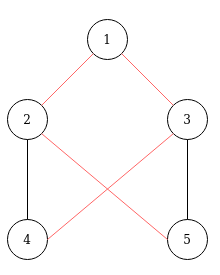
\includegraphics[scale=0.7]{p1-1.png}
\end{figure}

First and foremost, the set of edges highligted in the graph is non-cyclical, making it a tree. Further, since the path to each node is unique, said path is the shortest path to the afforementioned node. Finally, the tree cannot be created by a BFT by the following reasoing:

Since node 4 and 5 are connected to both nodes 2 and 3 in the graph. We cannot get node 5 connected only to node 2 and node 4 coddected only to node 3 if we use a BFT. This is because the BFT will always associate a child node the the first parend node the alogrithm visits, rather the nodes 4 and 5 will always be either attached to node 2 or to node 3. Thus any BFT starting at node 1 will give either the tree in Figure 2 or Figure 3 but not the on in Figure 4.
\begin{figure}[h]
	\caption{}
	\centering
	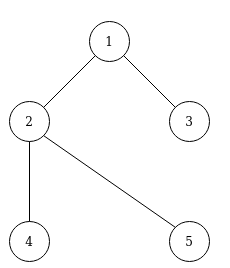
\includegraphics[scale=0.5]{p1-2.png}
\end{figure}
\begin{figure}[h]
	\caption{}
	\centering
	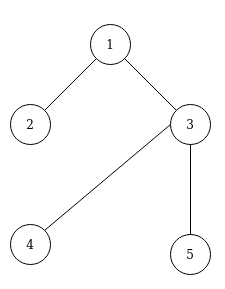
\includegraphics[scale=0.5]{p1-3.png}
\end{figure}
\begin{figure}[h!]
	\caption{}
	\centering
	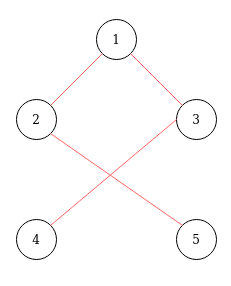
\includegraphics[scale=0.5]{p1-4.png}
\end{figure}


\pagebreak

\item \label{2} A \emph{simple $s \to t$ path} in a graph $G$ is a path in $G$ starting at $s$, ending at $t$, and never visiting the same vertex twice. Give an example graph (simple, undirected, unweighted) $G=(V,E)$ and vertices $s,t \in V$ such that DFS finds a path from $s$ to $t$ which is neither a shortest path nor a longest simple path. Detail the execution of DFS (list the contents of the queue at each step, and which vertex it pops off the queue), show the final $s \to t$ path it finds, show a shorter $s \to t$ path, and a longer simple $s \to t$ path.
\pagebreak

% YOUR ANSWER HERE
\begin{figure}[h!]
	\caption{Graph that will not return the correct path with DFT}
	\centering
	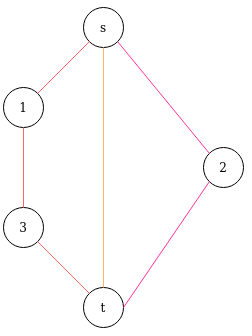
\includegraphics[scale=0.7]{p2-1.png}
\end{figure}

Assuming that the DFS will add nodes into the stack from left to right, the DFS starting at S will give and initial stack of [$s$]. We then pop S and add its children to the stack giving the stack [1, t, 2]. Then we pop the stack to get node 2 and add its children giving the stack [1, $t$, $t$]. Popping the stack again gives our destination $t$, resulting in the final path from $s \to t$ as the list [s, 2, $t$].

A shorter $s \to t$ path would be [$s$, $t$] and a longer one would be [$s$, 1, 3, $t$].
\pagebreak

\item \label{3} Give an example of a simple \emph{directed, weighted} graph $G=(V,E,w\colon E \to \mathbb{R})$ and vertices $s,t \in V$ such that Dijkstra's algortihm started at $s$ does \emph{not} find the shortest $s \to t$ path. \emph{Hint:} You will need to use negative edge weights. (Note: this shows that for finding shortest paths, the greedy choice property \emph{fails} in the presence of negative edge weights. Do you see why?)

% YOUR ANSWER HERE
\begin{figure}[h!]
	\caption{Graph that will not return the correct path with Dijkstra's}
	\centering
	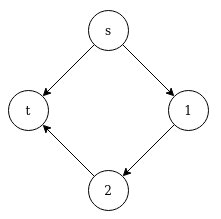
\includegraphics[scale=0.7]{p3-1.png}
\end{figure}

Starting at node 1, Dijkstra's algorithm will assign a value of 10 to $t$ and a value of 100 to 1. It will then select the node $t$ but since $t$ is the destination node, we will backtrack to $s$ and select node 1. From node 1 we set the value of node 2 to the value of node 1 plus 100 = 200. We then select node 2 since it is the only node available to select. From node 2 we, try to visit node $t$ but as it has already been visited, the algorithm will termiate and return the path [$s$, $t$]. The shortest path would be to select node 2 then node 2 then node $t$ to get a net weight of 0.

\pagebreak

\item \label{4} You have three batteries, with 4200, 2700, and 1600 mAh (milli-Amp-hours), respectively. The 2700 and 1600-mAh batteries are fully charged (containing 2700 mAh and 1600 mAh, respectively), while the 4200-mAh battery is empty, with 0 mAh. You have a battery transfer device which has a ``source'' battery position and a ``target'' battery position. When you place two batteries in the device, it instantaneously transfers as many mAh from the source battery to the target battery as possible. Thus, this device stops the transfer either when the source battery has no mAh remaining or when the destination battery is fully charged (whichever comes first). 

But battery transfers aren't free! The battery device is also hooked up to your phone by bluetooth, and automatically charges you a number of cents equal to however many mAh it just transfered. 
	
	The goal in this problem is to determine whether there exists a sequence of transfers that leaves exactly 1200 mAh either in the 2700-mAh battery or the 1600-mAh battery, and if so, how little money you can spend to get this result.
	\newpage
	\begin{enumerate}
	\item \label{4a} Rephrase this is as a graph problem. Give a precise definition of how to model this problem as a graph, and state the specific question about this graph that must be answered.

	Generate a graph such that each node is a 3 way tuple where each $(x,y,z)$ represends a valid permutation of the states of the 3 batteries as follows: $$(4200mAh, 2700mAh, 1600mAh)$$ For example, the first node would be $(0, 2700, 1600)$. Then connect each node base on whether or not a given node is a valid "next" state for the current node, eg the node $(0, 2700, 1600)$ would be connected to the nodes $(2700, 0, 1600)$ and $(1600, 2700, 0)$ as those are the only valid "next" staes of node $(0, 2700, 1600)$. Then weight each edge based on how much energy got transfered between one node and the next, eg the edge from node $(0, 2700, 1600)$ and node $(1600, 2700, 0)$ would have a weight of 1600 since 1600mAh got transfered from the 1600mAh battery to the 4200mAh battery. 

	Starting at the node $(0, 2700, 1600)$, we are looking for the shortest path to some node with the tuple $(a, 1200, c)$ or the tuple $(a, b, 1200)$ where $a, b$ and $c$ are arbitrary, vaild states of the 4200mAh, 2700mAh, and 1600mAh batteries respectively.
	\newpage
	\item \label{4b} What algorithm should you apply to solve this problem?
	
	Since we are looking for the shortest path through a graph, we should use Dijkstra's Algorithm to solve the problem.
	\newpage
	
	\item \label{4c} Apply that algorithm to the question. Report and justify your answer---both the sequence of steps and the total cost. To justify your answer here likely means you will have to detail the steps the algorithm takes.

	Final Answer: The path $$[(0,2700,1600), (2700,0,1600), (4200,0,100), (1500,2700,100),(1500,1200,1600)]$$ with a cost of \$84.

	See Figure 7

	Starting at Node A, the algorithm will assign a value of 1600 to node B and 2700 to Node C. It will then select Node B as it has the smallest value and assign $1600+2600=4200$ to Node D and $1600+1600=3200$ to Node E. The algorithm will then back track to Node C at it now has the lowest value and assign $2700+1500=3200$ to Node G and $2700+1600=3300$ to Node F. Since Node E and Node G are both the next smallest nodes, we pick one and continue. So the algorithm will pick node E and assign $3200+1600=4800$ to Node J and $3200+1600=4800$ to Node K. We then go to the next smallest node, Node G, and assign $3200+1500=4600$ to Node N and $3200+2700=5900$ to Node O. The next smallest one is Node F, so we assign $3300+1500=4800$ to Node L and $3300+1600=4900$ to Node M. Conitnuing this pattern, we will eventually arrive at Node R, which is the first node that we find that satisfies the criteria outlined in part a. The node will have a value of the sum of all the edges connecting it to the starting node, namely a value of $2700+1500+2700+1500=8400$ Thus the answer to the problem is to follow the path [(0,2700,1600), (2700,0,1600), (4200,0,100), (1500,2700,100),(1500,1200,1600)] with a final cost of \$84.

\begin{figure}[h!]
	\caption{Graph that will not return the correct path with DFT}
	\centering
	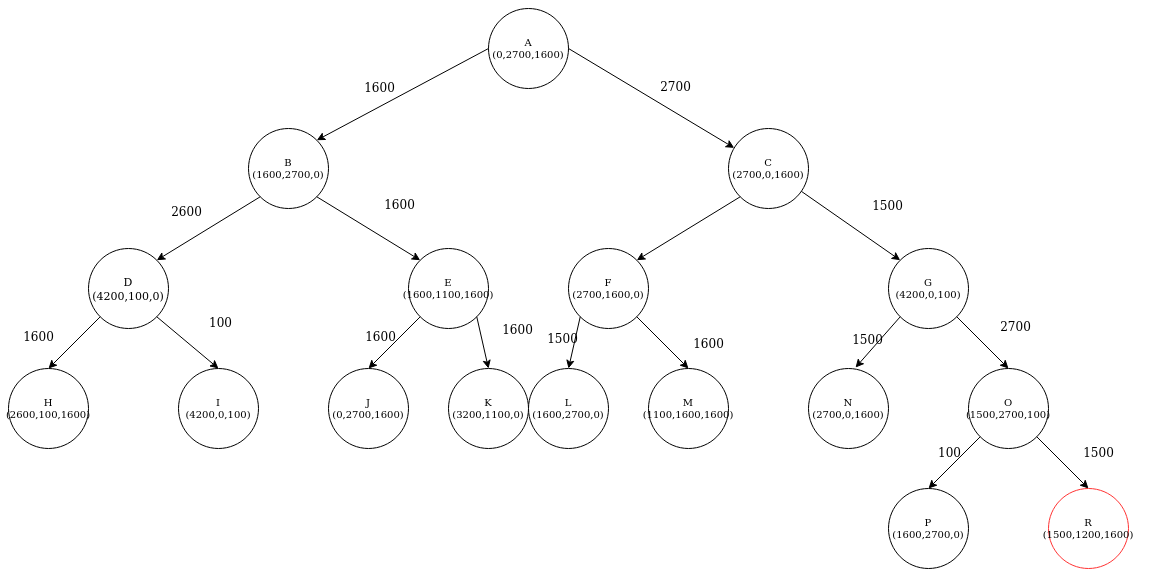
\includegraphics[scale=0.6, angle=90]{p4-1.png}
\end{figure}
	
	\end{enumerate}


\end{enumerate}


\end{document}


